\section{Measurement Techniques}
\subsection{Particle Time of Flight and Energy Determination}
\label{ToF_reconstruction}
The ToF of detected particles is used to distinguish between neutrons and photons and to determine neutron energy.
A particle's reconstructed position is used to determine direction of motion, which is then used to calculate the opening angle between pairs of detected particles.
Position and ToF are each determined using the timing of coincident signals from both PMTs of a detector.

The sum of the times required for scintillation light to travel from the point of scintillation to both PMTs is equal to the time required for the light to travel the full length of the scintillator, which is a constant for light that travels parallel to the length of the scintillator.
This is supported by data, shown in Fig.~\ref{fig:ConstPMTAvg}, which were produced from a series of tests in which a collimated $^{60}$Co source was placed at five different locations along a scintillator.
One of the two coincident photons emitted by $^{60}$Co reaches the scintillator and the other is detected by an auxiliary detector serving as the trigger. 
The photons incident on the scintillator have a spot size of less than 1~cm due to source collimation.
These events all have equal ToF, regardless of the source's position, because the coincident photons are emitted simultaneously and the distance they must travel is unchanged. 

In Fig.~\ref{fig:ConstPMTAvg}(a), it can be seen that the time required for the scintillation light to propagate through the scintillator has a large effect on the timing of each PMT alone, however, the average of the times of both PMTs is a constant, unaffected by the location at which the particle undergoes scintillation.
For this reason, taking the average of signals from two PMTs is advantageous because it removes the roughly 5~ns timing error that would otherwise exist due to the time required for scintillation light to propagate through the scintillator.
The requirement that there be coincident events in both of a detector's PMTs also aids in reducing noise.
\begin{figure}[h]
\centering
\subfloat[]{\hspace{-0.5cm}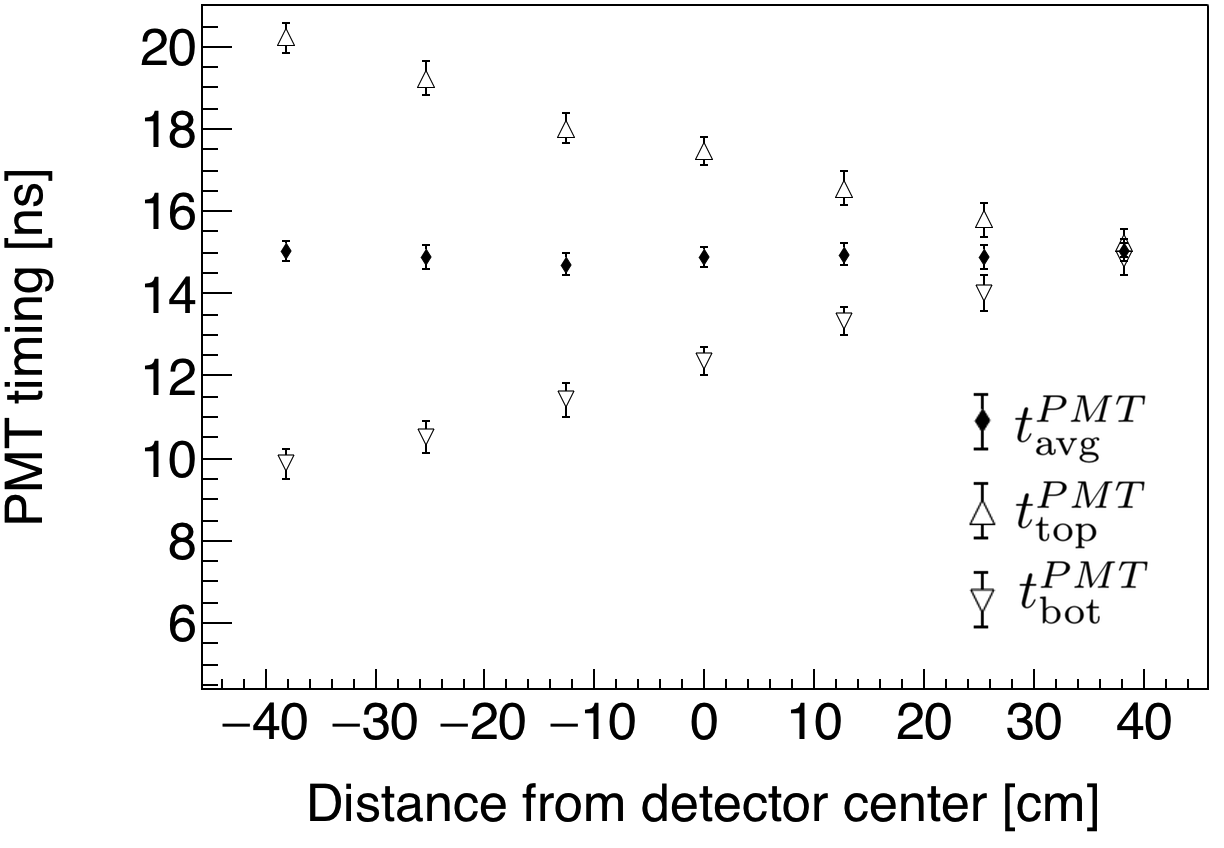
\includegraphics[width=0.65\textwidth]{Content/Methods/ConstPMTAvg.png}}

\subfloat[]{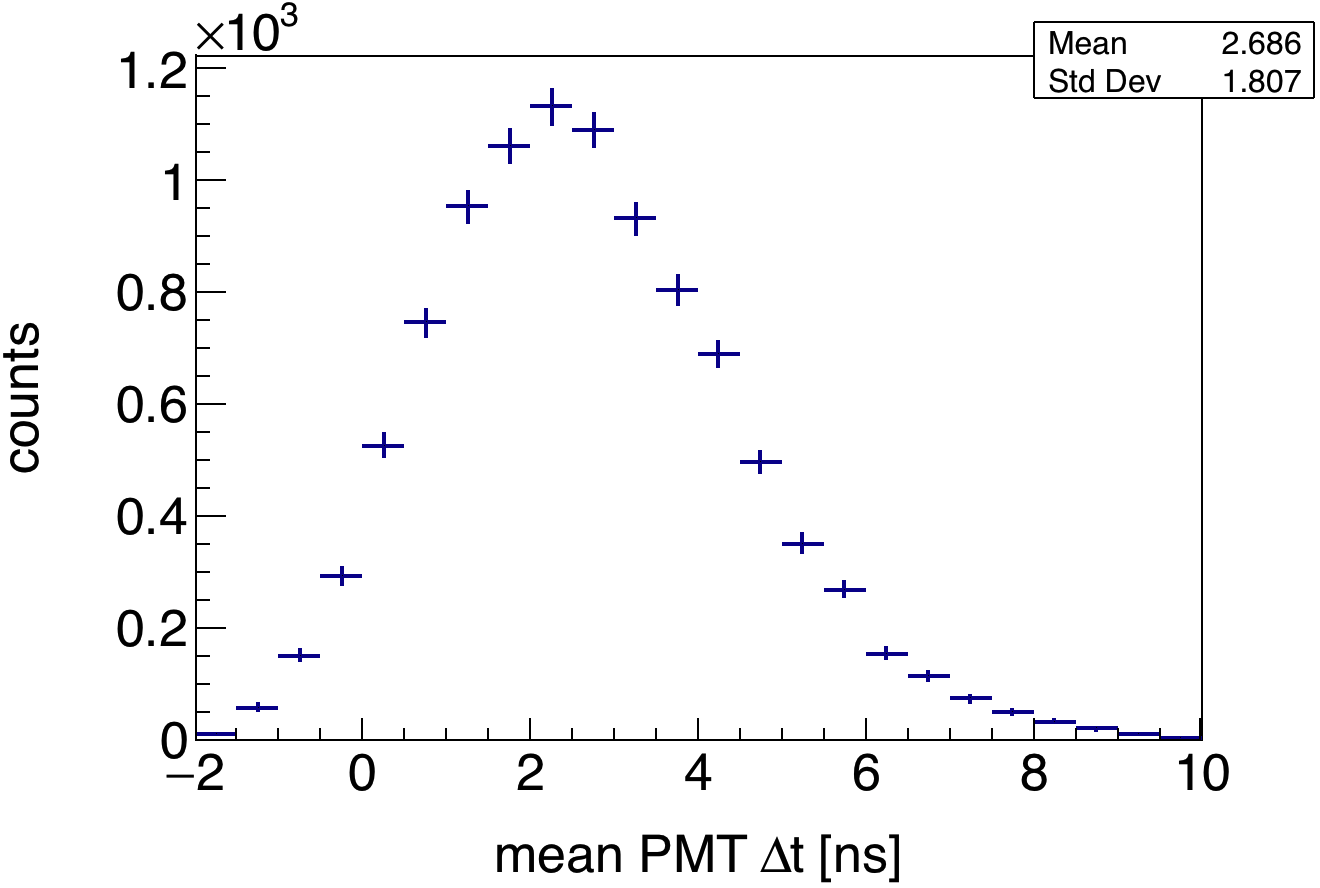
\includegraphics[width=0.65\textwidth]{Content/Methods/ConstPMTAvgProject.png}}
\caption{A collimated $^{60}$Co source is used to produce photon events with constant ToF at seven locations along the detector.
$^{60}$Co produces coincident photons, and one is detected by the scintillator and the other by a separate trigger detector.
 $\Delta t$ is the timing of a PMT signal relative to a signal from the trigger detector. 
 In (a), it can be seen that the average between signals from both PMTs does not depend on position.
By using the PMT average, there is a reduction in error due to the time required for scintillation light to travel through the scintillator.
The uncertainty in ToF measurements is equal to the standard deviation seen in (b), or about $\pm$2~ns, because all photons from the $^{60}$Co source have the same ToF.}
\label{fig:ConstPMTAvg}
\end{figure}

During photofission measurements, ToF is calculated by the following expression:
\begin{displaymath}
\text{ToF} = t^{PMTs}_{\text{avg}} - t_{\text{beam}} + C
\end{displaymath}
where $t^{PMTs}_{\text{avg}}$ is the average of the times of signals from both PMTs of a scintillator, $t_{\text{beam}}$ is the time of a signal provided by the accelerator at the beginning of each pulse, and $C$ is a constant timing offset.
Any process that produces a timing delay that does not change from pulse to pulse contributes to $C$, for example: \begin{itemize}
\item the time required for photons to travel from the bremsstrahlung radiator to the target
\item the propagation of signals through the wires connecting the PMTs
\item delays in the electronics
\item the signal transit time in the PMTs
\item the time required for scintillation light to propagate from the point of creation to both PMTs
\end{itemize}

The value of $C$, which may be different for each detector, is determined by comparing the timing spectra of the gamma flash produced by a non-neutron producing target made from aluminum, to that produced when no target is used.
The difference between these two spectra reveals a prominent peak in the ToF spectrum due to photons that scatter from the aluminum target.
These photons must travel 125~cm to reach the center of any detector and 130~cm to reach the top, for which it takes light 4.2~ns and 4.3~ns to travel, respectively.
The value of $C$ used for each detector is equal the value that places the time corresponding to the peak of the target-induced gamma flash at 4~ns.

Under the assumption that neutrons travel to the detectors unimpeded, the calculation of neutron energy from ToF is straightforward.
This assumption is validated through MCNP simulations that tested the frequency of the scattering of fission neutrons within the target and detector shielding, and is discussed in sections~\ref{subsection:targets} and \ref{subsection:detectors}.
Figure~\ref{fig:ErgUncertainty}(a) shows the relationship between neutron energy and ToF, and Figure~\ref{fig:ErgUncertainty}(b) shows the measurement uncertainty in neutron energy.
\begin{figure}[]
    \subfloat[]{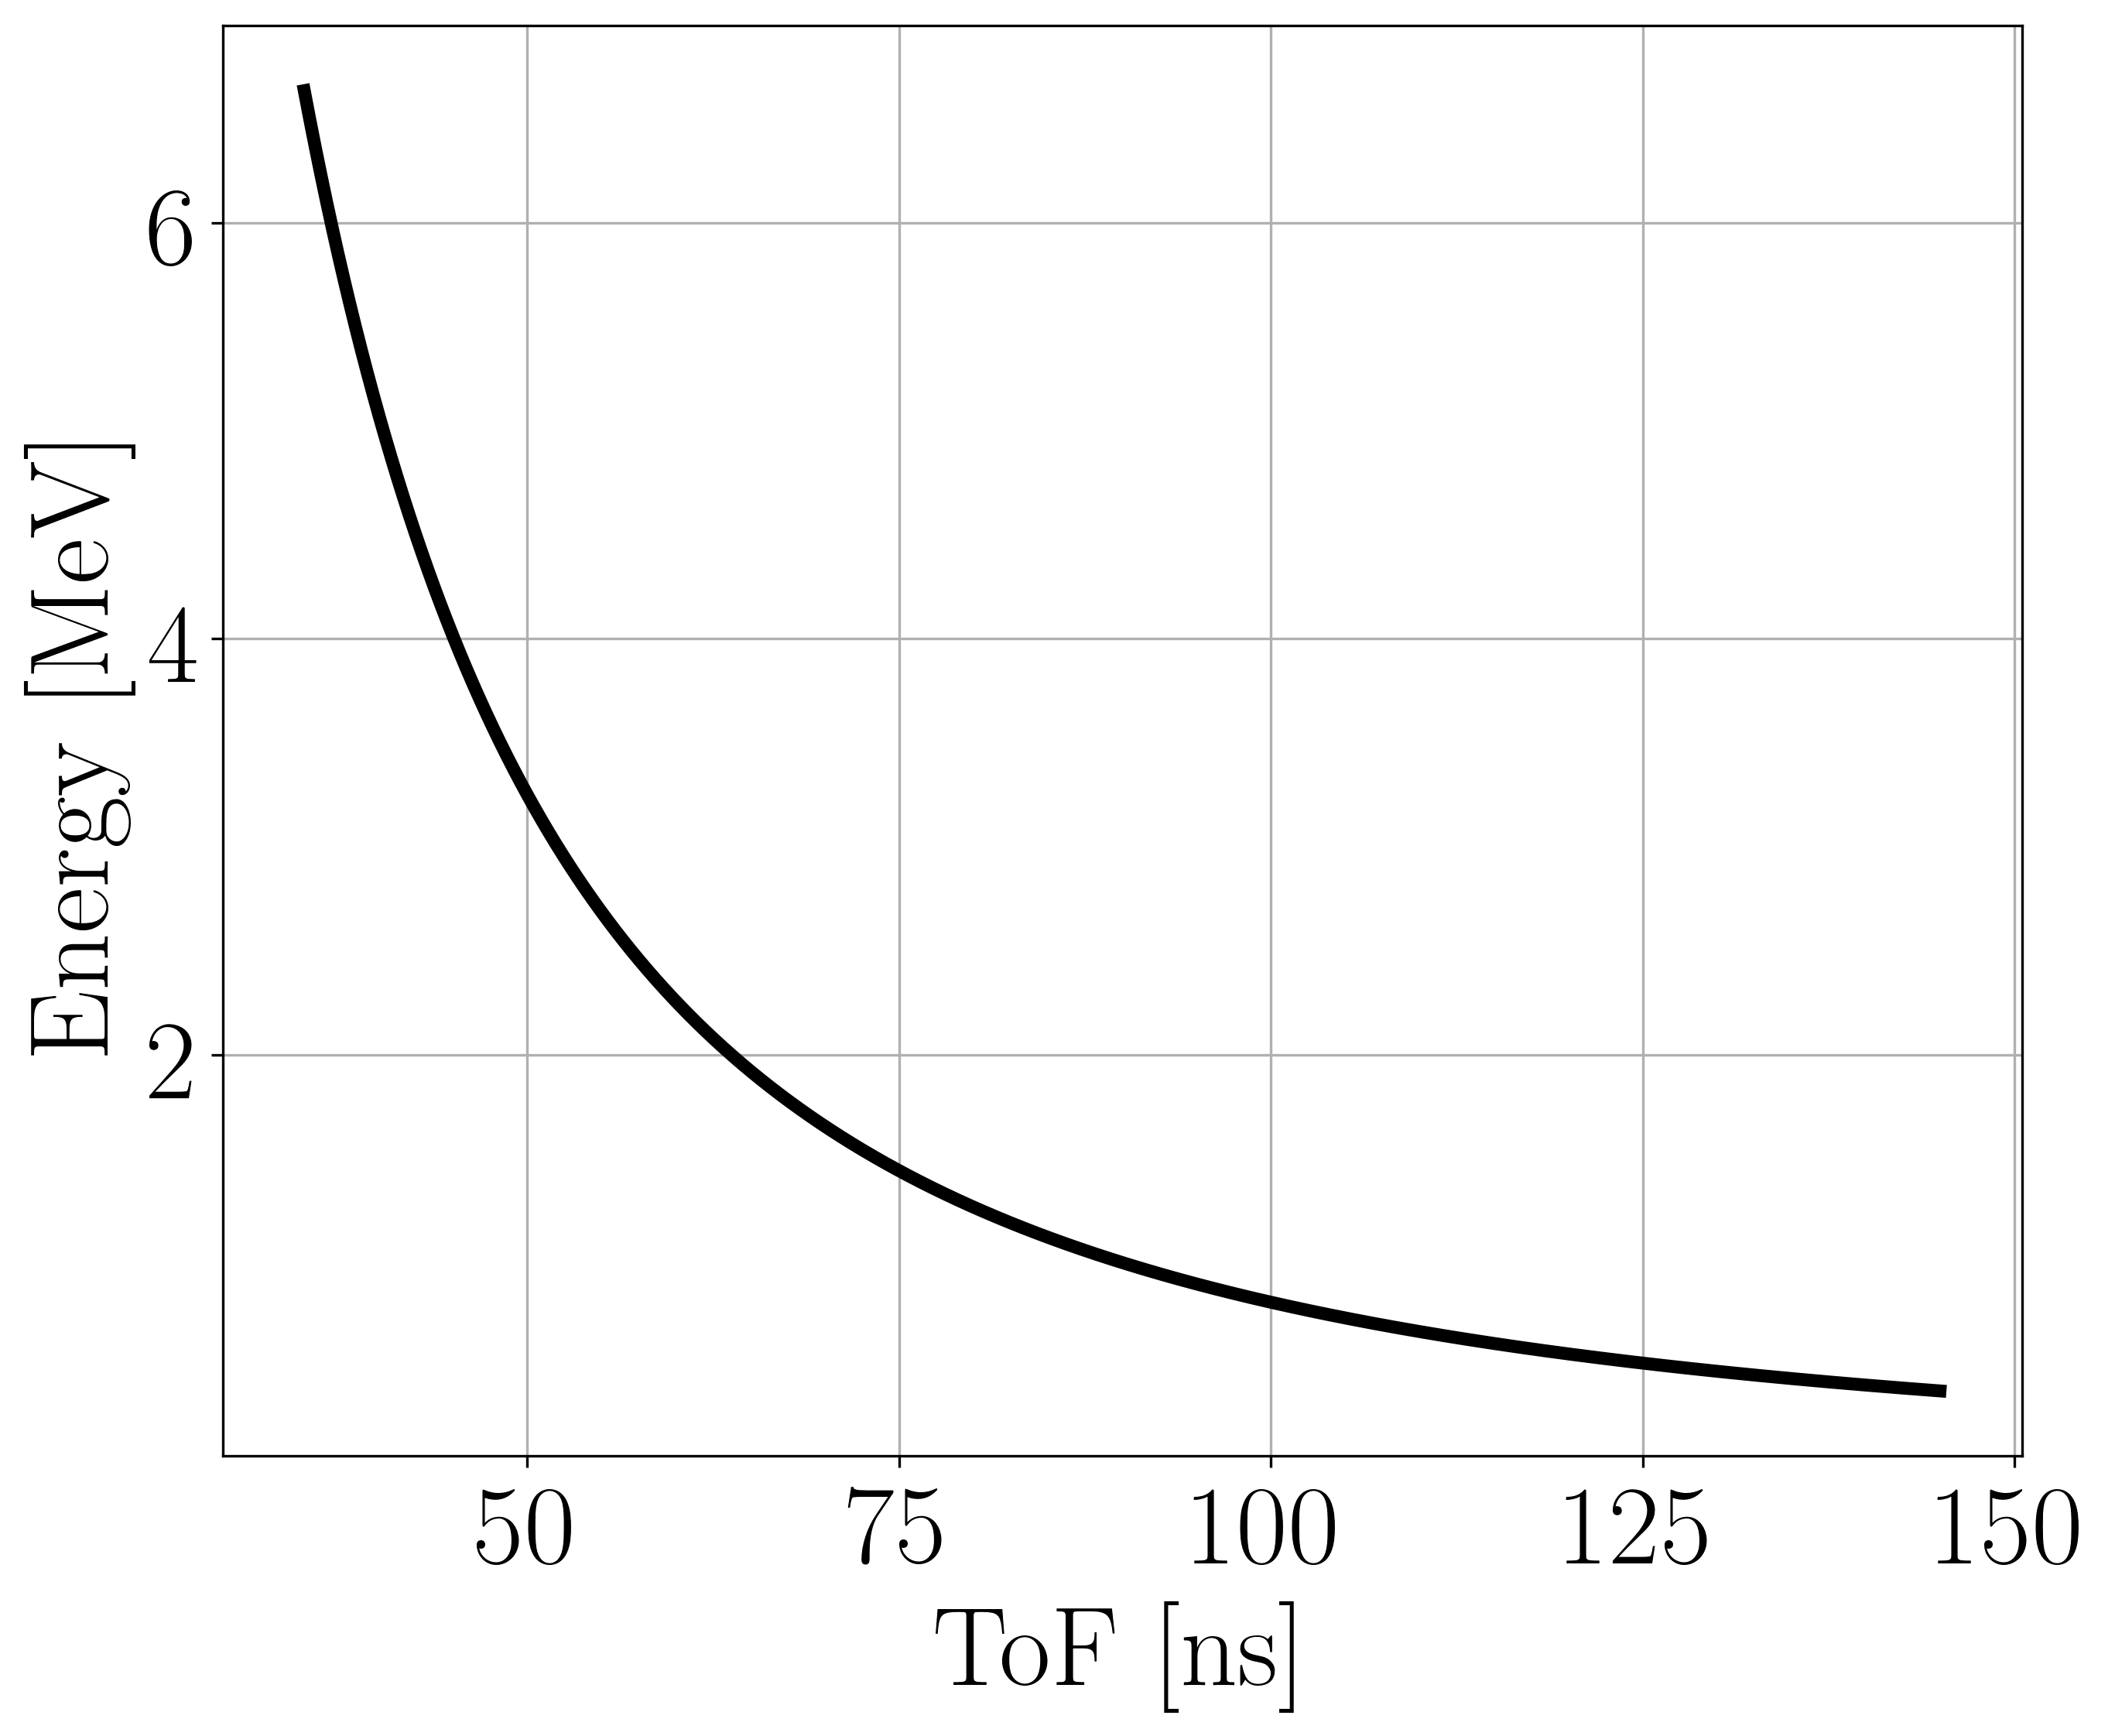
\includegraphics[width=0.5\textwidth]{Content/Methods/ToF2Erg.png}}
    \subfloat[]{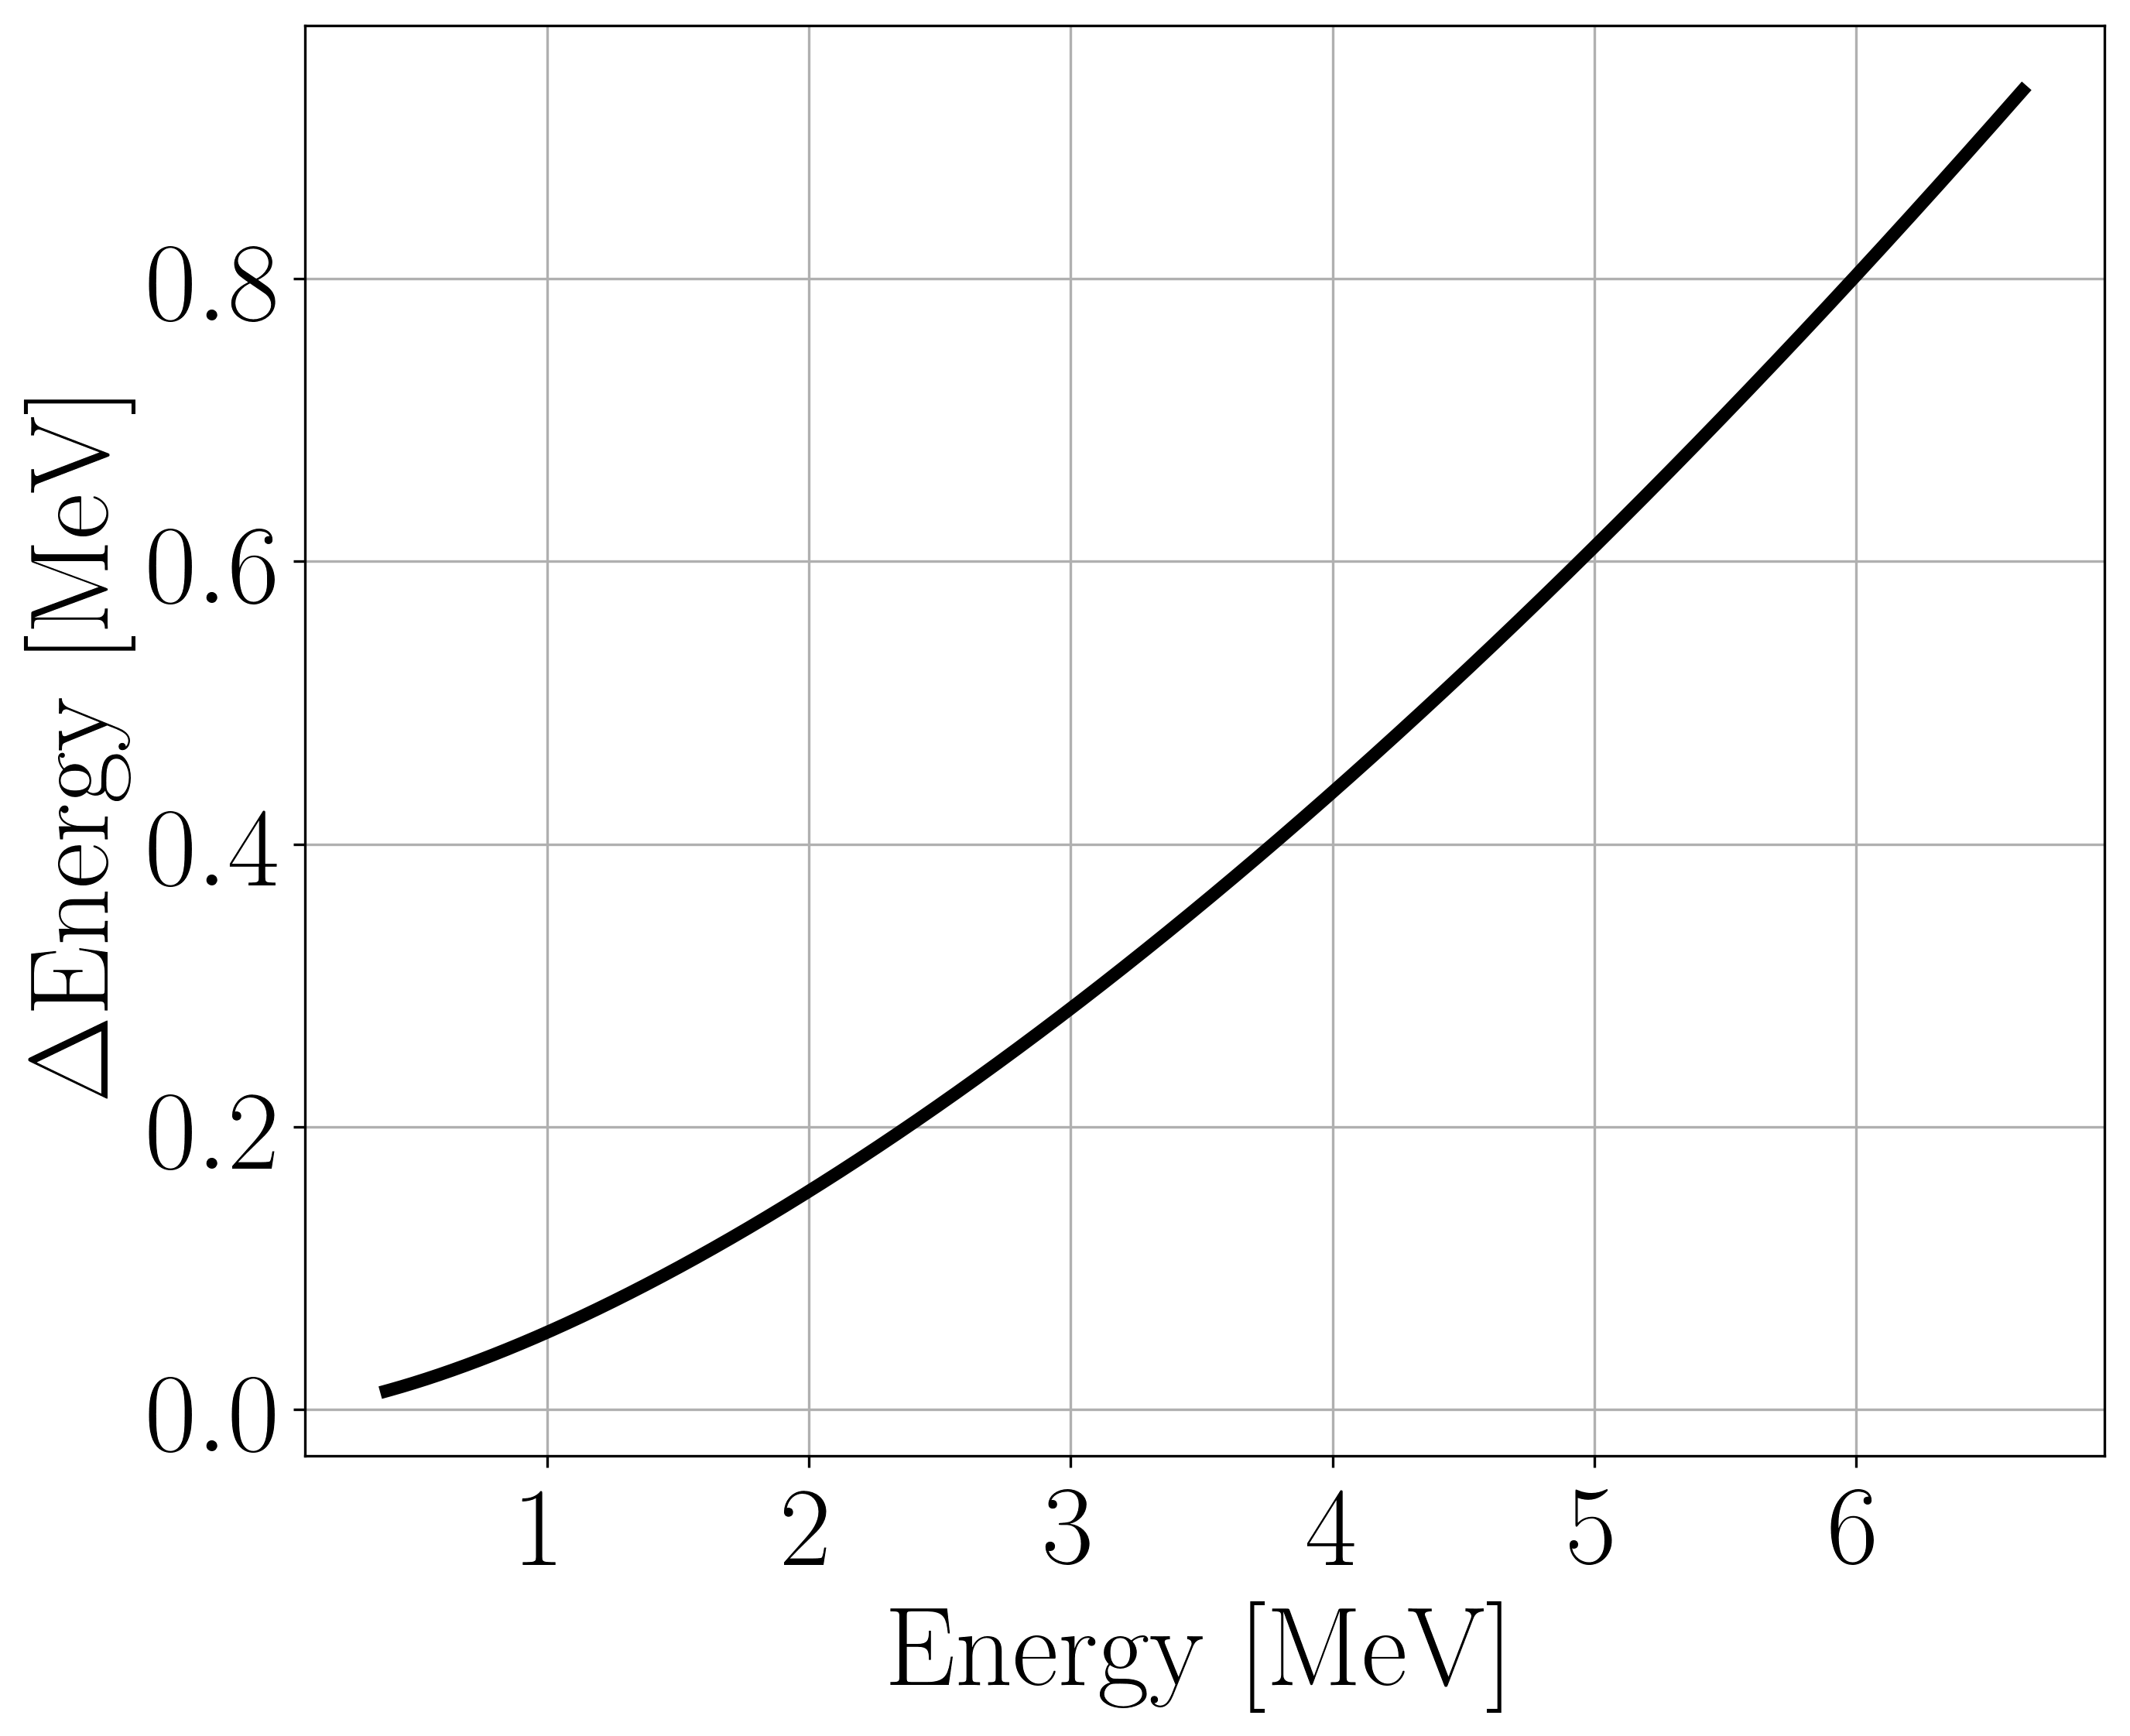
\includegraphics[width=0.5\textwidth]{Content/Methods/DeltaErg.png}}
    \caption{(a) Mapping from ToF to neutron energy: $E = \frac{8127}{ToF^{2}}$.
    (b) Uncertainty in neutron energy measurements as a function of measured neutron energy.}
    \label{fig:ErgUncertainty}
\end{figure}

\subsection{Particle Position Reconstruction}
Each detector is not capable of measuring the position of a detected particle along the axes parallel to its width (15.24~cm) or depth (3.81~cm), which contributes $\pm3^{\circ}$ to the total angular uncertainty.
The position of a detected particle along the 76.2~cm length of the scintillator is calculated using the timing difference of signals from both of a detector's PMTs.
Assuming that scintillation light travels from an initial point, let it be $x$~cm from the center of a scintillator, to both PMTs at a velocity that is constant with respect to the scintillator's length-wise axis, then the difference between the times at which the light will reach each PMT ($\Delta t^{PMTs}$) is given by:
\begin{equation}
\begin{split}
\Delta t^{PMTs} & = t^{PMT_1}-t^{PMT_2} \\ 
& = \frac{(L/2 + x) n_{\text{eff}}}{c} - \frac{(L/2-x) n_{\text{eff}}}{c} \\
& = 2x \frac{n_{\text{eff}}}{c}  \, .
\end{split}
\end{equation}
Solving for $x$ gives 
\begin{equation}
\label{eq:position}
x = \frac{c}{2n_{\text{eff}}} \Delta t^{PMTs} \, ,
\end{equation}
where $t^{PMT_{1}}$ and $t^{PMT_{2}}$ are the times of signals from each of a detector's PMTs relative to the accelerator gun pulse, $L$ is the length of the scintillator, $c$ is the speed of light, $n_{\text{eff}}$ is the effective index of refraction of the scintillation material.
A least squares linear fit between $x$ and $\Delta t^{PMTs}$ was performed on data gathered using coincident photons emitted by a collimated $^{60}$Co source, the procedure of which is mentioned in the previous section.
The resulting fit parameters, seen in Fig.~\ref{fig:PMTDifference}(b), are used to find the position of detected particles.
\begin{figure}[]
    \centering
    \subfloat[]{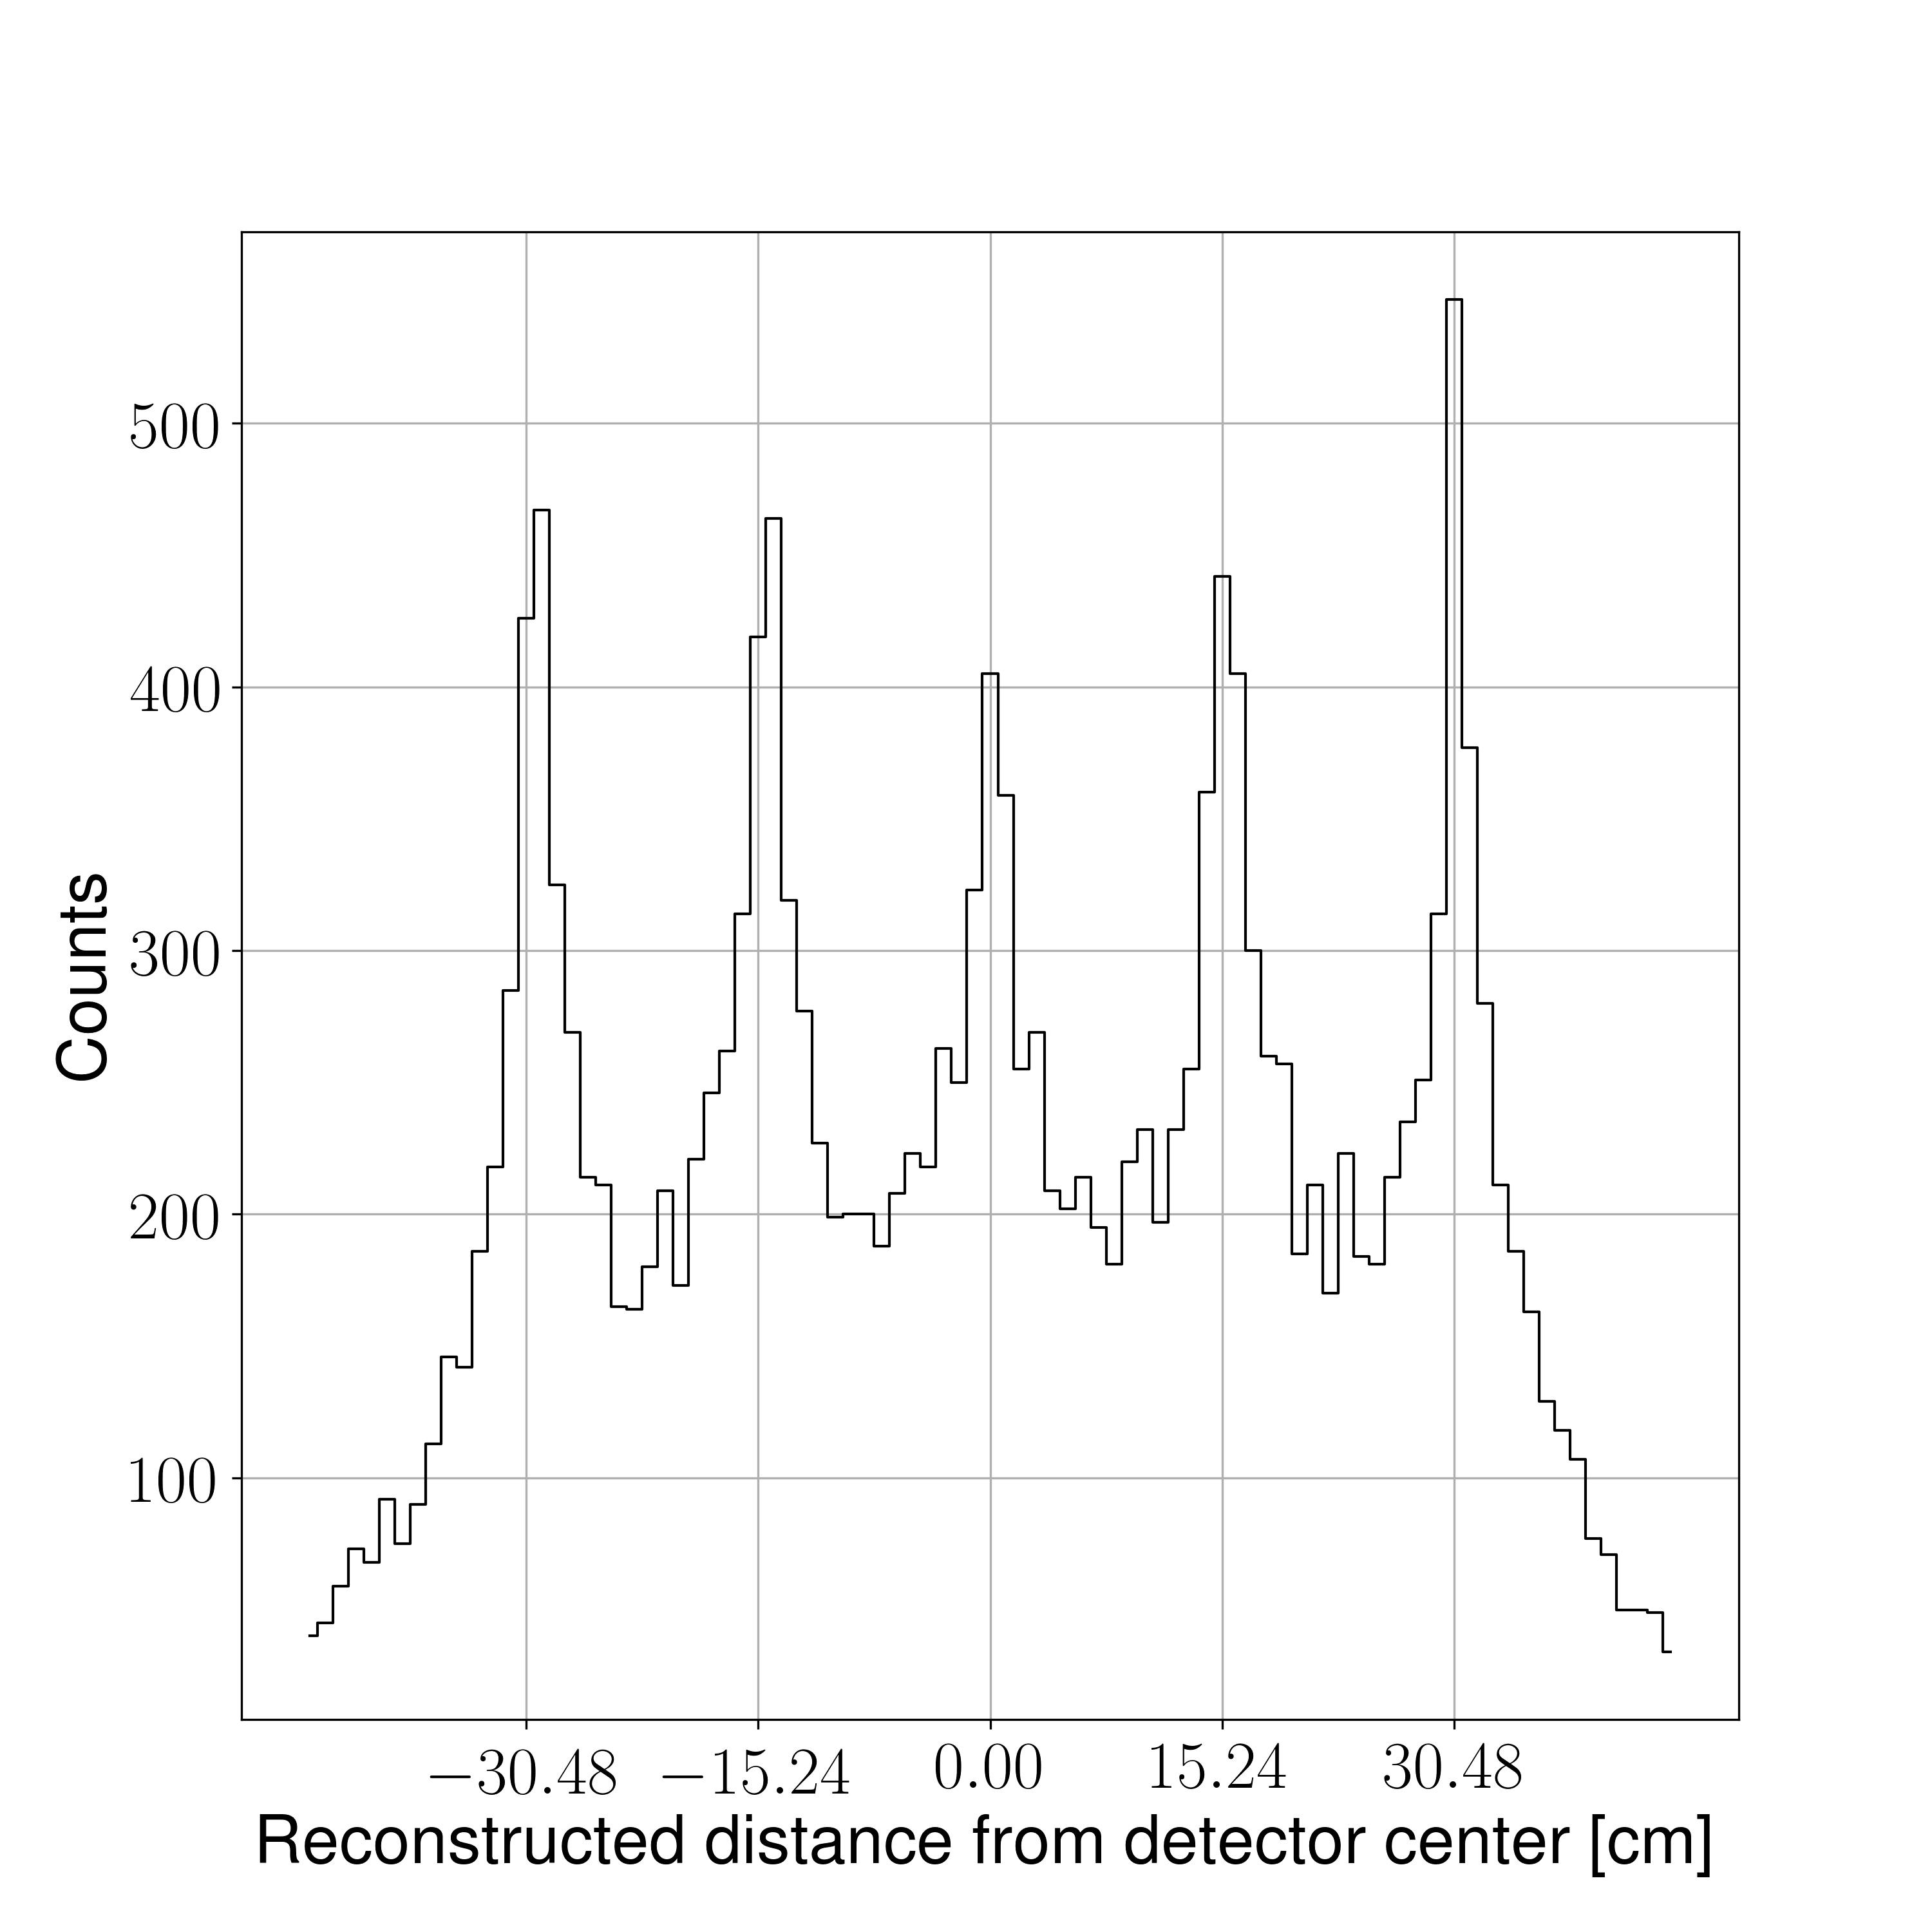
\includegraphics[width=0.5\textwidth]{Content/Methods/PMTDifference_hist.png}}
    \subfloat[]{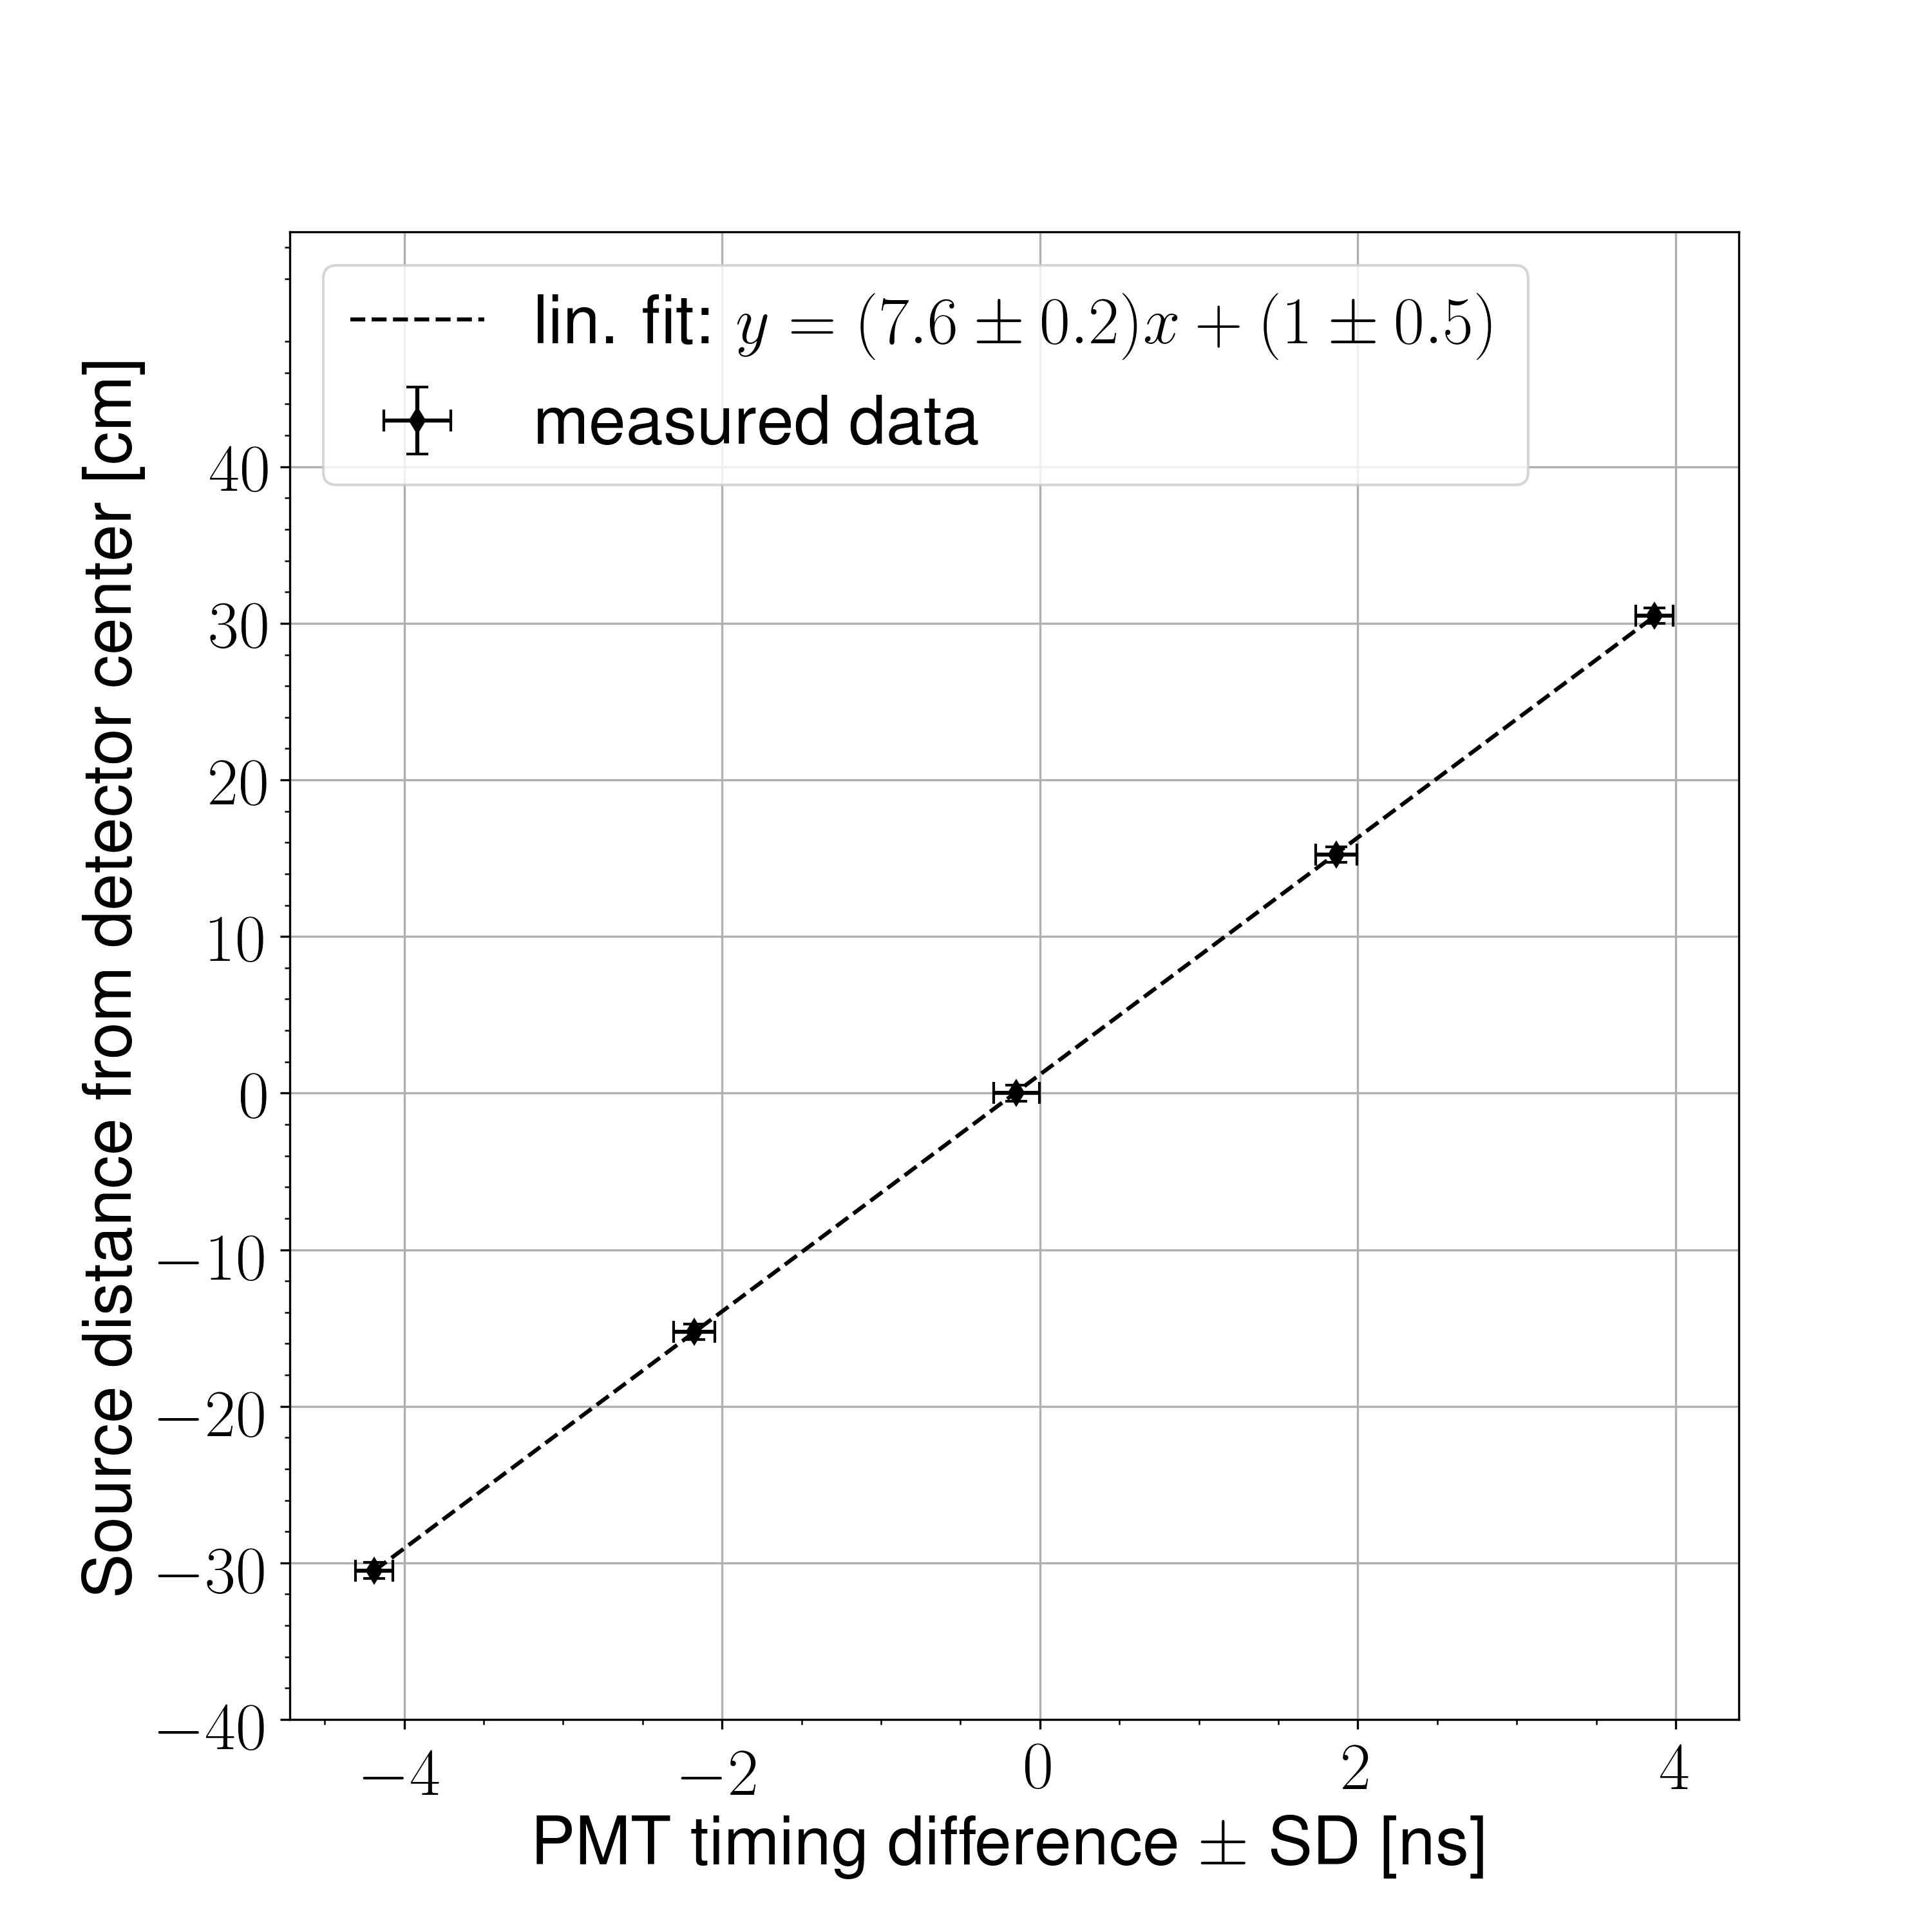
\includegraphics[width = 0.5\textwidth]{Content/Methods/PMTDifference.png}}

    \caption{
    A collimated $^{60}$Co source is used to produce photon events at five different positions along the scintillator.
    Aggregating the data from all five positions produces the five peaks seen in (a).
    The $\pm9$~cm width of each of these peaks is due to the measurement uncertainty in particle position.
    As seen in (b), the mean PMT timing difference of events at each position varies linearly with respect to the distance of the $^{60}$Co source from the center of the detector. 
    The result of a linear least squares fit to this data is used to calculate the position of detected particles along the length of each scintillator.
    }
    \label{fig:PMTDifference}
\end{figure}

Using the slope of the linear fit in Fig.~\ref{fig:PMTDifference}(b), along with Eq.~\ref{eq:position}, an effective index of refraction of the scintillation material is calculated to be 2.0.
This index of refraction is said to be ``effective" because its measurement is sensitive only to the scintillation light's average speed projected onto the axis parallel to the scintillator's longest dimension, which is equal to the intrinsic speed of light in the material only if the light is traveling parallel to the scintillator's length.
While the detection of scintillation light by both PMTs favors light paths which are parallel or nearly-parallel to the scintillator's length, there is some reflection of detected scintillation light from the boundaries of the scintillator.
This effect contributes to the $\pm9$~cm measurement uncertainty in particle position reconstruction, which is demonstrated in the widths of the peaks in Fig.~\ref{fig:PMTDifference}(a).
As a result of these effects, the actual index of refraction of PVT is 1.58, $\sim{20}\%$ less than the value measured here.


\subsection{Measurements with $^{252}$Cf}
\begin{figure}[h]
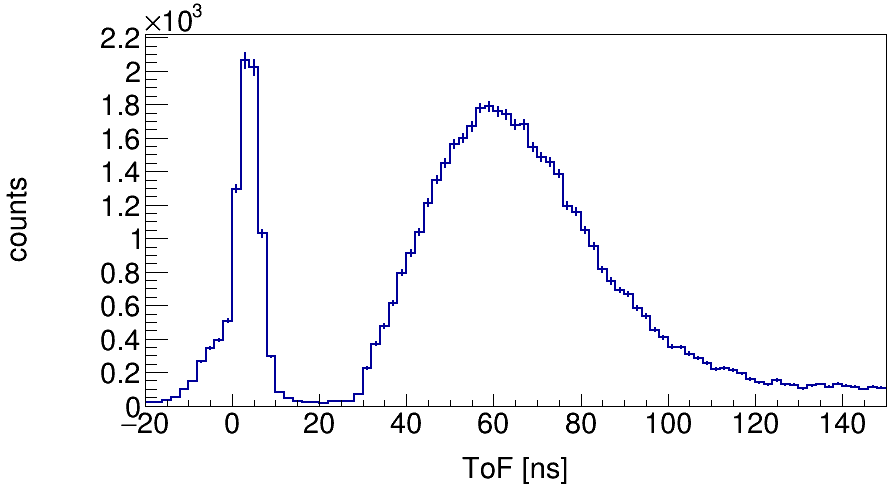
\includegraphics[width=0.75\textwidth]{Content/Methods/Cf252ToF.png}
\caption{Measured ToF spectrum from the SF of $^{252}$Cf.}
\label{fig:Cf252ToF}
\end{figure}
A $^{252}$Cf SF source was placed at the center of the detection system shown in Fig~\ref{fig:Facility} in order to measure the neutron-neutron opening angle distribution.
Several such past measurements have been performed (see refs~\cite{1975Cf252, Pozzi2014, 2008CF252, Verbeke2018}), and thus they served as a means to validate the methods used throughout this study.

The $^{252}$Cf SF source produces a cleaner ToF spectrum than photofission due to the lack of a photon beam (see Fig.~\ref{fig:Cf252ToF}), and, therefore, these measurements have a better signal to noise ratio.
Also, there is no concern over the detection of accidental neutron coincidences because the fission rate of the $^{252}$Cf source was about 3,500 fissions/s, making it highly unlikely that multiple fissions will occur during the electronic acceptance time window of 150~ns.
The beginning of the 150~ns neutron acceptance time window was triggered by a 2-fold coincidence, within a 4~ns window, between two separate 10$\times$10$\times$5 cm$^3$ plastic scintillators, one placed above and the other below the source at a distance of 30~cm.
Aside from this difference in the time window triggering mechanism, identical methods were used for both photofission and SF measurements.
\FloatBarrier